\documentclass[a4paper, 12pt]{report}
\usepackage{graphicx} % Required for inserting images
\usepackage[T1]{fontenc}
\usepackage[latin1]{inputenc}
\usepackage{graphicx}
\usepackage{titlesec}
\usepackage{xcolor}
\usepackage{amsfonts}
\usepackage{wrapfig}
\usepackage{amssymb}

\usepackage{glossaries}
\newtheorem{theorem}{Theorem}
\newtheorem{lemma}{Definition}
\newtheorem{proposition}{Proposition}
\newtheorem{proof}{Proof}
\usepackage{tikz}
\tikzstyle{mybox} = [draw=black, thin, rectangle, rounded corners, inner ysep=5pt, inner xsep=5pt, fill=orange!20]

\usepackage[a4paper, top=2cm , bottom=2cm , right=2cm , left=2cm ]{geometry}

\graphicspath{ {images/} }

\titlespacing{\title}{10pt}{50pt}{50pt}
\titlespacing{\chapter}{0pt}{10pt}{10pt}
\titlespacing{\section}{10pt}{5pt}{10pt}

\title{
    \textbf{  \Huge{  MODELING AND  CONTROL OF\\ 
    CYBER-PHYSICAL SYSTEMS } }\\
    \textit{Lecture notes}
}
\author{Carlo Migliaccio}
\date{AA 2023/2024}

\begin{document}
\maketitle
\tableofcontents

\part{Modeling of Cyber-Physical systems}
\chapter{Introduction}
\section{Some definitions}
\noindent
\textbf{Definition} (Helen Gill, 2006) "Cyber-Physical systems are physical, biological, and engineered systems whose operations are integrated, \textbf{monitored, and/or controlled} by a \textbf{computational core}. Components are \textbf{networked} at every scale. Computing is deeply embedded into every physical component, possibly even into materials. The computational core is an embedded system, usually demands real-time response, and is most often distributed"\\

\noindent Roughly speaking a CPS is a \textbf{collection of devices} that:
\begin{enumerate}
    \setlength\itemsep{-.5em}
    \item compute
    \item inter-communicate
    \item interact with the physical word
\end{enumerate}

\begin{figure}[h]
    \centering
     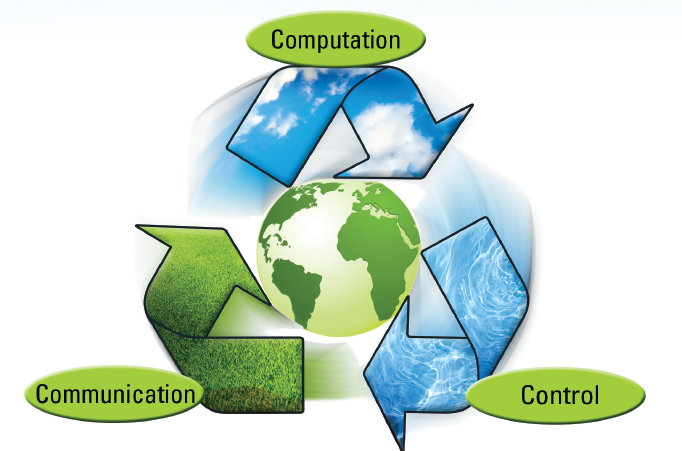
\includegraphics[width=0.6\textwidth]{images/CPS.png}
    \caption{Three Dimensions of CPSs}
    \label{fig:enter-label}
    \end{figure}
    
\noindent 
At this point, we can distinguish in this scenario two layers for CPS: (1) The \textbf{Cyber Layer} which is linked to the computation and communication issues, (2) the \textbf{Physical Layer} deals with the interaction of the devices with the physical word.\\
\vspace{2cm}
%-------------------------------------------------------------

\section{Some examples of CPS}
\noindent
Examples of Cyber-Physical systems could be:
\begin{itemize}
    \item \textbf{Automotive vehicles}: in a car you can find hundreds of sensors, actually we have a computational core, are interconnected in some way (eg. CAN), moreover several feedback-control systems can be find;
    \item \textbf{Teams of mobile robots} that aim to get a target. Robots collaborate to achieve a goal that can be: the exchange of information for example; 
    \item \textbf{Wireless sensor networks} in order to monitor and area (indoor localization without a GPS)
\end{itemize}

%-------------------------------------------------------------
\section{Enabling Technologies and related problems}
\noindent
We can wonder: "How can we deploy CPS?". The answer is by using: 
\begin{enumerate}
    \setlength\itemsep{0em}
    \item \textbf{Embedded systems}: hardware and software integrated within mechanical and electrical systems
    \item \textbf{Sensors and Actuators} for monitoring and control purposes
    \item \textbf{Communication Networks} for example Wireless communication
\end{enumerate}
Despite the \textbf{implementation} it's not too much expensis it raises several issue: at first the \textbf{Vulnerability} which is linked to the \textbf{Safety} of the overall system.

%-------------------------------------------------------------
\section{Mathematical models for CPS}
\noindent
We can modelize a Cyber-Physical System by using: 
\begin{itemize}
      \setlength\itemsep{0em}
    \item \textbf{Basic  Models}: continuos-discrete time LTI systems
    \item \textbf{Hybrid models}: they can describe the interaction between devices and the physical layer including both continuous and discrete events; 
    \item \textbf{Systems under adversarial attacks}: a CPS could be attacked in order to manipulate the exchanged information;
    \item \textbf{Multi-agent systems}: networks of intercommunicating \textit{agents} which may collaborate to reach a \textit{common goal}: \textbf{Consensus}.
\end{itemize}
\subsection*{Hybrid systems}
In order to \textbf{model the presence of physical events} that can change the dynamics, we can consider \textbf{hybrid systems}, also known as  \textbf{switched linear systems}. We can describe them by using the following formalism:
\vspace{1cm}
\begin{large}
    \begin{align*}
    &x(k+1)=A_{q_k}x(k)+B_{q_k}u(k)\\
    &y(k)= C_{q_k}x(k)+D_{q_k}u(k) 
\end{align*}
\end{large}

\vspace{3cm}
for $k=0,1,...$
\begin{itemize}
    \setlength\itemsep{0em}
    \item $x(k)$ is the continuous state
    \item $q_k \in \{1, 2, ..., Q\}$ is the discrete state or {\color{red} mode}, if $q_k \neq q_{k+1}$ then at the time $k$, the dynamics changes, there is a \textbf{switch} for the system
    \item The parameters denoted with \textbf{$A_{q_k}, B_{q_k}, C_{q_k}, D_{q_k} $} are associated witch the {\color{red} active submodel}, the parameters are {\color{blue} piecewise constant}. For this reason the hybrid systems could be seen as a particular case of LTI systems.
\end{itemize}
\noindent
Some examples of hybrid systems could be: a bouncing ball,  a robot moving with obstacles (which are items of the physical layer) in a room etc.

\subsection*{Modeling the presence of attacks}
An attack in the framework of CPS can be modeled as an additive term either on the actuator or the (distributed) sensors.
\begin{align*}
    &x(k+1)=Ax(k)+Bu(k)+b(k)\\
    &y(k)=Cx(k)+Du(k)+a(k)
\end{align*}
Where we indicate with: 
\begin{itemize}
    \setlength\itemsep{0em}
    \item $b(k)$ the attacks on the actuators
    \item $a(k)$ the attacks on the sensors
\end{itemize}

\noindent
We focus only on the term $a(k)$ which can alter the dynamics of the system. We can't model the attacks as a \textit{disturbance/noise} as we could face them by using some techniques of the classical control theory (eg. Loop shaping).\\
A "good attack" can't be modeled in a proper way like a disturbance, but fortunately as the sensors are distributed, the attacks can be done only on a subset of them. There are in the common case \textbf{sparse attacks.}
Our reference model to develop the theory is then the following: 
\begin{align*}
    &x(k+1)=Ax(k)+Bu(k)\\
    &y(k)=Cx(k)+Du(k)+{\color{red}a(k)}
\end{align*}




%---------------------------------------------------------------------
\chapter{Secure estimation of CPSs state under adversarial attacks}
\section{State estimation and Observabilty}

\noindent
Let us consider the LTI system (without input):
\begin{align*}
    &x(k+1)=Ax(k)\\
    &y(k)=Cx(k)
\end{align*}

\noindent
$y(k)\in \mathbb{R}^q$, $x(k) \in \mathbb{R}^n$, $A\in\mathbb{R}^{n,n}$, $C\in\mathbb{R}^{q,n}$\\

\noindent
The \textbf{State estimation} is the procedure by which we can \textbf{recover} the state $x(k)\in\mathbb{R}^n$ of the system from measurements $y(k)$ for $k=0, 1, 2, ...$. \textbf{Note that...} every element of the vector $y(k)$ is a measure from a sensor, and so we have $y_i(k)\in\mathbb{R}$.\\
We can say that a system is \textbf{Observable} if exists a finite time $T\in\{0,1,...\}$ such that \textbf{$x(0)$} can be recovered from the measurements $y(k), \quad k=0,1, ..., T-1$. \\

\noindent
But why only $x(0)$? Let us compute $y(0), ..., y(T-1)$ to verify this fact: 
\begin{flalign*}
&y(0)=Cx(0)
\\&y(1)=Cx(1)=CAx(0)
\\&y(2)=Cx(2)=CA^2x(0)
\\&...
\\&y(T-1)=...=CA^{T-1}x(0)
\end{flalign*}
At this point by using the vectorial notation, we have:
\begin{equation*}
    \begin{pmatrix} y(0)\\ y(1)\\ y(2)\\   \vdots\\    y(T-1) \end{pmatrix} 
    =
    \begin{pmatrix}
        C\\ CA \\ CA^2 \\ \vdots \\ CA^{T-1} 
    \end{pmatrix} x(0)
\end{equation*}

$\mathcal{O}_T$ = 
$\begin{pmatrix}
    C\\ CA \\ CA^2 \\ \vdots \\ CA^{T-1} 
\end{pmatrix}$ 

$\in\mathbb{R}^{qT, n}$ where if $T=n$ we call 
$ \mathcal{O}_n$ 
the \textbf{Observability matrix}.\\
\noindent
When the equation 
\begin{equation*}
    \begin{pmatrix} y(0)\\ y(1)\\ y(2)\\   \vdots\\    y(T-1) \end{pmatrix}= \mathcal{O}_T  x(0) 
\end{equation*}
has a \textbf{unique solution} the system is observable.
At this point, we distinguish two different cases: 
\begin{itemize}
    \setlength\itemsep{0em}
    \item $qt<N$ the system is \textit{underdetermined}
    \item $qt\geq N$ and $rank(\mathcal{O}_T)=n$, then we can (pseudo)invert it. In particular if  $qT=n$ then $$x(0)=\mathcal{O}_T^{-1}y(k)$$ otherwise if $qT>n$ then $$x(0)=(\mathcal{O}_T^T\mathcal{O}_T)^{-1}\mathcal{O}_T^Ty(k)$$
\end{itemize}
Where we call \textbf{Moore-Penrose pseudoinverse} the matrix 
    $\mathcal{O}_T^{\dagger}=(\mathcal{O}_T^T\mathcal{O}_T)^{-1}\mathcal{O}_T^T$

\begin{theorem}{(Kalman, 1960)}
    An LTI system is observable if and only if rank($\mathcal{O}_n$)=n
\end{theorem}
In general there are two approaches for the state estimation: 
\begin{itemize}
    \setlength\itemsep{0em}
    \item \textbf{static approach}: solving the equation like we have just seen.
    \item \textbf{dynamic approach}: by using a \textbf{Luemberger Observer} that allow us to recover the state after a bunch of steps. 
\end{itemize}

\section{Secure state estimation}
\noindent
In this section we make a try to expand the concept of \textbf{Observability and state estimation} when we have attacks on the sensors, and so the additive term $a(k)$ in the output equation.
\begin{align*}
    &x(k+1)=Ax(k) \\
    &y(k)=Cx(k)+a(k)
\end{align*}
\textbf{Assumption} The term $a(k)\in\mathbb{R}^q$ is  {\color{red}\textbf{sparse}} in the sense that no more than $h\ll q$ of its elements are non-zero. By using the $l_0$-norm, $\lVert a\rVert_0\le h$. \\

We refer to \textbf{Secure state estimation} when we want recover the state $x(0)$ from sensors' measurements $y(k), k=0,1,...$ and \textbf{unknown attacks} $a(k)$. (As we said we are not able to model attacks in a proper way, we wouldn't have a different theory and several techniques to face the problems related to them).

Let us anylize the mentioned problem by spotting the differences that occurs in the case of attacks: 
\begin{flalign*}
&y(0)=Cx(0)+a(0)
\\&y(1)=Cx(1)=CAx(0)+a(1)
\\&y(2)=Cx(2)=CA^2x(0)+a(2)
\\&...
\\&y(T-1)=...=CA^{T-1}x(0)+a(T-1)
\end{flalign*}
Then 
\begin{equation*}
    \begin{pmatrix} y(0)\\ y(1)\\ y(2)\\   \vdots\\    y(T-1) \end{pmatrix} 
    =
    \begin{pmatrix}
        C\\ CA \\ CA^2 \\ \vdots \\ CA^{T-1} 
    \end{pmatrix} x(0) + 
     \begin{pmatrix} a(0)\\ a(1)\\ a(2)\\   \vdots\\    a(T-1) \end{pmatrix} 
\end{equation*}
where we have {\color{red}qT equations} for {\color{red}$n+qT$ unknowns}! That would indicate potentially \textbf{infinitely many solutions}.\\
{\color{blue}Despite this observation if we add the hypotesis that the vector containing the attack is \textbf{sparse}, in some situations we could have a unique solution to this problem. 
}
\begin{lemma}
    \large{
    We say that $h$ errors are \textbf{correctable} after T steps if its possible to recover any $x(0)$ given $y(0), ..., y(T-1)$ under the condition $\lVert a \rVert_0 \le h$, for each $k=0,..., T-1$}.
\end{lemma}
This corresponds to ask that the problem \\

\hspace*{-5mm}
\begin{tikzpicture}
\node [mybox] (box){%
    \begin{minipage}{.96\textwidth}     %Larghezza del box
           \begin{equation*}
    \begin{pmatrix} y(0)\\ y(1)\\ y(2)\\   \vdots\\    y(T-1) \end{pmatrix} 
    =
    \begin{pmatrix}
        C\\ CA \\ CA^2 \\ \vdots \\ CA^{T-1} 
    \end{pmatrix} x(0) + 
     \begin{pmatrix} a(0)\\ a(1)\\ a(2)\\   \vdots\\    a(T-1) \end{pmatrix} 
     \quad \textrm{s.t.} \quad  \lVert a \rVert_0 \le h,  k=0,..., T-1
\end{equation*}
    \end{minipage}
};
\end{tikzpicture}%


\noindent
had a \textbf{unique solution}.



\noindent
Now we have to face with two problems: 
\begin{enumerate}  
    \setlength\itemsep{0em}
    \item Under \textbf{which conditions} can I solve the proposed problem?
    \item \textbf{How can I solve} it?
\end{enumerate}

\noindent
\section{Well-Position of the problem (Static case)}
Let us analyze the problem in a very particular case, that is when the system we want to ovbserve is \textbf{static}. That is the matrix $A\in \mathbb{R}^{n,n}$ is the identity matrix $\mathbb{I}_n$. This corresponds to state that $x(k+1)=x(k)=x$ (remember that we have no input $u(t)$).\\
In this case the observability matrix has a very simple form, in particular it is equal to the matrix $C\in\mathbb{R}^{q,n}$. We have that the problem becomes: 
{   \large{
    $$y=Cx+a \quad \textrm{s.t.} \quad \lVert a \rVert_{0} \le h$$ }
}

\noindent
It is useful to give these formal definitions:\\
\begin{lemma}[h-sparsity]
    A vector is said to be \textbf{h-sparse}, if  $\lVert a \rVert_0 = h  $
\end{lemma}

\begin{lemma}[Support]
    Given $a\in \mathbb{R}^q$ we denote with $Supp(a)=\{i: a_i \ne 0\}$, the set of i such that the i-th component of the vector is a non-zero number.
\end{lemma}

\noindent
{\color{red} \textbf{How the attack could be done in order to not to be 'detectable'?}}
 Let's consider an $a=Cw, \quad w \in \mathbb{R}^n, w \ne 0$ and assume it is that $\lVert Cw \rVert_0 \le h$ (for the assumption we made). We sobstitute in the equation and obtain:
$$y=Cx+Cw=C(x+w) \quad \textrm{s.t.} \quad \lVert Cw \rVert_0 \le h$$
Actually, if such $w$ exixts, the \textbf{attack is feasible} and so not detectable. This property depends strongly on the property of the matrix $C$.\\
Fortunately we have a \textbf{proposition} that provide us with an equivalence to determine the \textbf{resilience} of the system to h  attacks.


\vspace{0.3cm}

 \hspace*{0mm}
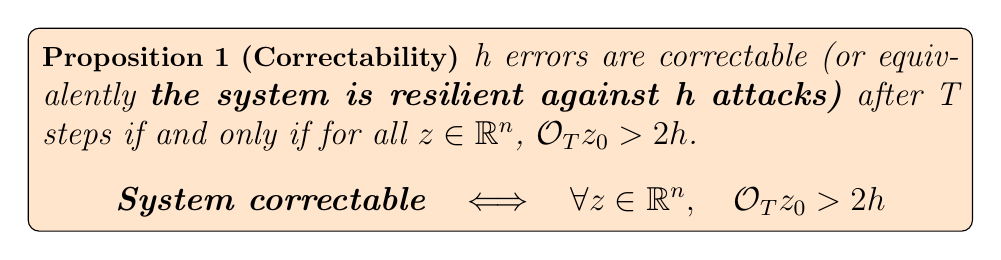
\begin{tikzpicture}
\node [mybox] (box){%
    \begin{minipage}{.96\textwidth}
          \begin{proposition}[Correctability]
    \large{
    h errors are correctable (or equivalently \textbf{the system is resilient against h attacks)} after T steps if and only if for all $z\in\mathbb{R}^n$, $\lVert \mathcal{O}_Tz \rVert_0 > 2h$.}
    $$\textrm{\textbf{System correctable}} \quad \Longleftrightarrow \quad \forall z \in \mathbb{R}^n , \quad \lVert \mathcal{O}_Tz \rVert_0>2h$$
\end{proposition}
    \end{minipage}
};
\end{tikzpicture}%

\noindent
In the static case the Proposition 1 becomes: $$\textrm{\textbf{System correctable}} \quad \Longleftrightarrow \quad \forall z \in \mathbb{R}^n , \quad \lVert Cz \rVert_0>2h$$
\begin{proof}
    As this is a characterization property we have to proof the proposition in the two direction $\Leftarrow$ and $\Rightarrow$. We give this proof for the static case, but the procedure for the more general case is analogue.
    \begin{itemize}
        \item {\Large{\textbf{[Proof of $\Leftarrow$] }}}
        {\color{blue} Assuming that 
        $\forall z \in \mathbb{R}^n$ we have $\lVert Cz \rVert_0 > 2h $ we want to demonstrate that h errors are correctable}, that is the problem has a unique solution.  As in many situation we want to demonstrate the uniqueness of something, we can go on \textbf{by contraddiction}. In particular assume that $y=Cx+a$ s.t. $\lVert a \rVert_0 \le h$ has got two different solutions: 
        $$\begin{pmatrix}
            x'\\ a'
        \end{pmatrix} and \begin{pmatrix}
            x''\\a''
        \end{pmatrix}$$

        then we have that $y=Cx'+a' \quad \textrm{s.t.} \quad \lVert a' \rVert_0 \le h$ but also $y=Cx''+a'' \quad s.t. \quad \lVert a'' \rVert_0 \le h $. $Cx'+a'=Cx''+a''$ $\Longleftrightarrow C(x'-x'')=a''-a'$ But due to the fact that $a'$ and $a''$ are h-sparse we can obtain by substracting them a vector which is \textbf{at most} 2h-sparse. 
        We have finished because we found a contradiction , that is, $\exists  z \in \mathbb{R}^n, \lVert Cz \rVert_0 \le 2h$. In this case $w=a'-a''$
        
        \item {\Large{\textbf{[Proof of $\Rightarrow$] }}}{\color{blue} Assuming that h errors are correctable,  we want to demonstrate that 
        $\forall z \in \mathbb{R}^n$ we have $\lVert Cz \rVert_0 > 2h $ }. Similarly the former case,  we can demonstrate the property by contradiction assuming that $\exists w \in \mathbb{R}^n \quad \lVert Cw \rVert_0 \le 2h$. We can write such $Cw$ like a sum of two (at most) h-sparse vectors $g_1$ and $g_2 \rightarrow Cw=g1+g2$. But we can also say that $Cw=g_1+g_2 \longleftrightarrow Cw-g_1=g_2=C 0+g_2 $. In this way we are saying that we have \textbf{two distinct solutions}, this is in contradiction with our hypotesis. \texttt{QED}
    \end{itemize}
\end{proof}

\noindent
The proposition that has just been proved is very powerful, but how are we able to try for all $z$ that the statement is valid? In the great majority of the situations is easier to provide a \textbf{counter-example}.\\
Now we are going to do some example and then to provide (at least) a necessary condition for well-position of the problem of correctability. 

\subsection{Some examples}
{\color{orange}\subsubsection{Example 0: a "naive" example}}
Consider that we have $C=\mathbb{I}_n$, $q=n$, $h=1$, $n=3$. In this case the output equation is: 
\begin{align*}
    &y_1=x_1\\
    &y_2=x_2\\
    &y_3=x_3
\end{align*}
As we can see the system is \textbf{perfectly observable} because each measurement of $y$ gives an element of the state, but suppose that we know that there is an attack ($h=1$), but we don't know where. If one of the measurement is corrupted, there is no way to recover the state of the system $\Rightarrow$ $C$ is not correcting h errors $\Rightarrow$ the system is not resilient to h attacks. In an intuitive way we can say that we could add more sensors to improve the situation, it is 'the path' that follows the next example.

{\color{orange}\subsubsection{Example 1: add more sensors (increase q)}}
At this point we change the (sensing) matrix $C$ by adding new measurements, so
$$C=\begin{pmatrix}
    1 &0 &0\\0& 1& 0\\0& 0 &1 \\ 1& 0& 0 \\ 0& 1& 0
\end{pmatrix}$$
What has changed here is that we have \textbf{two more }sensors. We have a duplication of $C_1$ and $C_2$ (we indicate with $C_i$ the i-th row of C). If $y_1=C_1x=y_4=C_4x$ and $y_2=C_2x=y_5=C_5x$ than we can state that the attack is on the sensor 3. But\textbf{ what if either $y_1 \ne y_4$ or $y_2 \ne y_5$}? We have no way to know which sensor has been attacked. If I switched off this couple of devices I can't observe anymore one of the component of the state vector. \\
This was only an \textbf{intuitive way} to understand this fact. How can we formalize it? 
We can say that the couple $(C_1, C_2)$ has a \textbf{non trivial kernel}. That is the equation:
$$\begin{pmatrix}
    1&0&0\\0&1&0
\end{pmatrix}z=\begin{pmatrix}
    0\\0
\end{pmatrix}$$
has a non zero solution. In particular a solution could be $z=\begin{pmatrix}
    0\\0\\\alpha
\end{pmatrix}$ such $z$ produces 
$$Cz=\begin{pmatrix}
    0\\0\\\alpha\\0\\0
\end{pmatrix} \quad \alpha \in \mathbb{R}$$ which due to the fact which is 1-sparse, is \textbf{in contradiction} with the proposition.\\
Conclusion: \textbf{even this matrix does not correct h=1 error $\Rightarrow$ the system \textbf{is not} resilient}!

{\color{orange}\subsubsection{Example 2: more mixed measurements}}
Freezing the other parameters, let us change again the matrix $C$ in the following way: 
$$C=\begin{pmatrix}
    1&0&0\\0&1&0\\0&0&1\\1&1&1\\1&-1&1
\end{pmatrix}$$
It is quite clear that there is a triple of rows of C which are linearly dependent, specifically $C_5=C_4-2C_2 \Rightarrow$ the triple has a non trivial kernel. By doing simple algebraic steps we desume that a solution could be  $z=\begin{pmatrix} 
    \alpha\\0\\-\alpha
\end{pmatrix}$ which generates a 2-sparse $Cz$ we have again a contradiction! Conclusion: \textbf{C is not resilient}. 

{\color{orange}\subsubsection{Example 3: linearly independent measurements}}
Now we provide the following $C$ matrix: 
$$C=\begin{pmatrix}
    &1&0&0\\&0&1&0\\&0&0&1\\&1&1&1\\&1&2&-1
\end{pmatrix}$$
In this case all the triples are linearly independent, this cause the relative kernel to be trivial $\rightarrow$ there is no way to produce a counter-example. 
Conclusion: this  $C$ matrix corrects h=1 error.

\subsection{A necessary condition for well-position}
Let $C\in \mathbb{R}^{q,n}$, $rank(C)=n$ and $q>n$, it is quite clear that any subset $\Omega$ composed by $n-1$ rows  has got a non trivial kernel. This implicates that the sparsity is not larger than $q-(n-1)$, that is $2h < q-(n-1)$ or equivalently $h \le q-n$. From which I can recover the following inequality: $$q\ge 2h+n$$
It is immediate to understand that if I want to correct $h=1$ error with $n=3$, we need at least of $q=5$ sensors.

This fact bring us to state that: 
\begin{itemize}
    \item Large $q$ is not sufficient for \textbf{resilience} 
    \item On the other hand there is a \textbf{minimum q} which I need to correct a certain number $h$ of errors.
\end{itemize}

\section{Reformulation of $y=Cx+a \quad \textrm{s.t.} \quad    \lVert a \rVert_0 \le h$}
\noindent
The second question to answer is: \\
{\begin{center}
\textbf{
    How can we solve the problem $y=Cx+a \quad \textrm{s.t.} \quad    \lVert a \rVert_0 \le h$?}
\end{center}} 
The problem can be reformulated as follows:
{   \large{
        $$\min_{x\in\mathbb{R}^n, a\in\mathbb{R}^q} \lVert a \rVert_0 \quad \textrm{s.t.} \quad y=Cx+a$$
    }
}\\
It can be proved that \textbf{if the system is resilient to h attacks the solution to this problem corrects h errors}. Unfortunately, even this form of the problem has its drawbacks: 
\begin{itemize}
    \item As the problem is a combinatorial one, is \textbf{not feasible} (NP-Hard)
    \item The \textbf{objective function} which contains an $\ell_0$ norm is \textbf{not convex, non continuous and non differentiable in 0}
\end{itemize}
The solution is going in the direction of \textbf{convex relaxation}: 
\begin{enumerate}
    \item In the objective function, we choose to relax $\lVert a \rVert_0$ with its \textbf{best CONVEX approximation} $\lVert a \rVert_1$; it is \textsc{Convex}, \textsc{Continuous} but \textsc{Non differentiable in 0} (we can face this problem);
    \item In the real world, we must take into account the noise that could appear in the equation $y=Cx+a$ and so it becomes $y\approx Cx+a$, this leads to the \textbf{Least Squares (LS) problem} $$\min{ \frac{1}{2}\lVert y-Cx-a \rVert_2^2}= 
    \min{\frac{1}{2}\Bigg\lVert y - \begin{pmatrix}
        C & I 
    \end{pmatrix}\begin{pmatrix}
        x\\
        a
    \end{pmatrix} \Bigg\rVert}$$ 
\end{enumerate}

Combining this two approximations, due to the fact we want to minimize both the terms, the \textbf{resulting problem to solve} is: 

\hspace*{-5mm}
\begin{center}
    \begin{tikzpicture}
    \node [mybox] (box){%
        \begin{minipage}{.80\textwidth}
                %Qui testo
                {
                \color{black}
                \Large{
                    $$
                    \min_{x\in\mathbb{R}^n, a\in\mathbb{R}^q}{\frac{1}{2}\Bigg\lVert y - \begin{pmatrix}
                        C & I 
                    \end{pmatrix}\begin{pmatrix}
                        x\\
                        a
                    \end{pmatrix} \Bigg\rVert}+\lambda\lVert a \rVert_1, \quad \lambda>0
                    $$
                }}
                
        \end{minipage}
    };
    \end{tikzpicture}%
\end{center}



\subsection{Why $\ell_1$-regularization promotes sparsity?}
\begin{figure}[h]
    \centering
    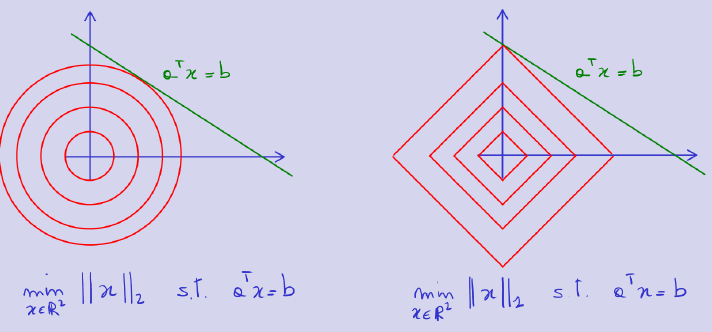
\includegraphics[scale=0.8]{images/Sparsity.png}
    \caption{$\ell_p$-norms and sparsification}
    \label{fig:enter-label}
\end{figure}
In the approximation we have just made, we have considered the $\ell_1$-norm. But why it is the best we could do? Let us consider to solve the problem $$\min_{x\in\mathbb{R}^2} \lVert x \rVert_2 \quad  \textrm{s.t.} \quad a^Tx=b$$ 
The term $\lVert x \rVert_2=k, k\in\mathbb{R}$ is a circle in the plane. We start from $k=0$, and we increase it until we reach the line to satisfy the (linear) constraint. The solution we obtain is certainly not sparse because it is of the form $x^*=(x_1^*, x_2^*)$ both non-zero real number.\\
\noindent
On the other hand if we consider the problem: 
$$\min_{x\in\mathbb{R}^2} \lVert x \rVert_1 \quad  \textrm{s.t.} \quad a^Tx=b$$ 
we note that the solution we can find (by using the same method as before) is sparse. We have seen in an intuitive way that $\ell_2$-norm takes the components of the solution close to zero in a "democratic way", in other words without 'reset' any component. At the opposite the $\ell_1$-norm push to zero \textbf{only some components} making a selection among them $\longleftrightarrow $ this promotes \textbf{"sparsification"}.\\

\noindent
{
    \color{blue}
    [Note that we have just showed a trivial way to understand why we have chose one regularization instead of another. The topic would require a more accurate and rigorous explanation, which we don't care.]
}

\subsection{Some observations}

\subsubsection{The problem has a connection with LASSO}
The problem we found to solve after applying \textbf{relaxation} is very similar to the problem of \textbf{LASSO} (Least Absolute Shrinking and Selection Operator) in fact in its original formulation we have: 
$$\min_{x\in\mathbb{R}^n} \frac{1}{2}\lVert Ax-y \rVert_2^2+\lambda\lVert x \rVert_1$$
but this give an entire sparse solution. In our problem only a piece of the solution is sparse, whose linked to attacks $a$, so we can see our problem as a "\textbf{Partial LASSO}" because we have \textbf{no regularization} on the term $x$ of the solution $\begin{pmatrix}
    x\\a
\end{pmatrix}$.

\subsubsection{The problem has a connection with "Compressed Sensing"}
The problem
 $$
    \min_{x\in\mathbb{R}^n, a\in\mathbb{R}^q}{\frac{1}{2}\Bigg\lVert y - G\begin{pmatrix}
        x\\
        a
    \end{pmatrix} \Bigg\rVert}+\lambda\lVert a \rVert_1, \quad \lambda>0,
    \quad 
    G=\begin{pmatrix}
        C & I 
    \end{pmatrix}
    $$
as the $G$ matrix has more columns than rows, is a \textbf{fat matrix} and without regularization the problem has infinitely many solutions. We can consider the $y$ a \textbf{linear compressed measurement} vector.
The problem of \textbf{recover a sparse vector from compressed linear measurement} has a strong connection with the \textsc{Compressed sensing} problem. Also here we have a \textbf{"Partial Compressed Sensing"} as only a part of the solution is sparse.\\

\noindent
{
\large{
    \color{red}
    After a "long journey" we have understood that for the \textbf{secure state estimation of CPS under adversarial attacks} we have to solve a \textbf{Partial LASSO} problem. For this reason we seek a way to solve it $\Rightarrow$ Iterative Algorithms
    }
}
    
\section{IST: an algorithm for LASSO}
\noindent
{\color{blue}
\textit{
    \textbf{Premise} In this course we will not see any black box technique, we will go through the direction of \textbf{iterative algorithms} to solve the LASSO problem.\\
    \noindent
    In the framework of \textbf{Convex Optimization} one of the most used algorithms (also in Data Science/Machine Learning...) is the \textbf{Gradient Descent Algorithm}. But in the LASSO we have a $\ell_1$-regularization, which is not differentiable in 0. We can't even avoid to consider it because we want to reach the (global) \textbf{minima}. We wonder if using an approximation could be the solution (eg. \textbf{subgradients}), however again this not produce a \textit{sparse solution}. 
}\\
}

\noindent
Once the proper promises have been done, we can introduce this algorithm for solving the \textbf{(sparse) optimization problem} of LASSO. 
The algorithm is called \textbf{Iterative Shrinkage/Thresholding (IST)} and it is a variant of the \textit{Descent Gradient Algorithm}. After the definition and a general description, we are goingo to list the steps of the algorithm itself. Initially we consider the original LASSO problem
$$\min_{x\in\mathbb{R}^n} \frac{1}{2}\lVert Ax-y \rVert_2^2+\lambda\lVert x \rVert_1$$ in which we call $F(x)=\lVert Ax-y \rVert_2^2$ the Least-Squares functional. Moreover we know that $\nabla F(x) = A^T(Ax-y)$.\\

\noindent
\textbf{Definition (Shrinkage/Thresholding operator)} The \textbf{Shrinkage/Thresholding operator} $\mathbb{S}_{\alpha}$ is a component wise operator $\mathbb{S}_{\alpha}: \mathbb{R}^p \rightarrow \mathbb{R}^p, \alpha >0$. For any $x_i\in \mathbb{R}$:
\begin{equation*}
    \mathbb{S}_{\alpha}(x_i) =
        \begin{cases}
            x_i-\alpha & \text{if $x_i$>$\alpha$} \\
            x_i+\alpha & \text{if $x_i$ < -$\alpha$}\\
            0 & \text{if $ \lvert x_i \rvert \le \alpha$}\\ 
        \end{cases}
\end{equation*}



\hspace*{-5mm}
\begin{tikzpicture}
\node [mybox] (box){%
    \begin{minipage}{.96\textwidth}

    \textbf{\Large{IST Algorithm}}\\
        \begin{enumerate}
            \item Initialization: $x_0\in\mathbb{R}^p$, e.g. $x_0=0$
            \item For $k=0,..., T_{max}$
            \Large{
            \begin{equation*}
                x(k+1)=\mathbb{S}_{\lambda \tau} \left[ x(k)-\tau\nabla F(x(k))
                \right]
            \end{equation*}
            }
        \end{enumerate}
    \end{minipage}
};
\end{tikzpicture}%

\vspace{0.5cm}
\noindent
The parameter $\tau$ has to be "small enough" so that the algorithm works as desidered. It has been demonstrated that the algorithm converge to the minimum of the LASSO functional $\frac{1}{2}\lVert Ax-y \rVert_2^2+\lambda\lVert x \rVert_1$. The \textbf{iterative nature} and simplicity of this method, makes it adaptable also for: \textbf{dynamic} and \textbf{distributed} systems.

\subsection{Derivation of IST Algorithm} 
Let us do a quick RECAP of the latest notions we introduced...\\
Generally speaking, when we have some measurements $y=A\tilde{x}+\eta$ where $\tilde{x}$ is the \textbf{true vector} to recover, we are able to find an \textbf{estimate} of it by solving the problem 
$$x^{*} = \textrm{arg} \min_{x\in \mathbb{R}^n} \frac{1}{2}\lVert y-Ax \rVert_{2}^{2}$$
also known as the \textbf{Least Squares (LS)} problem, where the obtained $x^*$ is the estimate of the true vector. How can we solve this problem?\\
The \textbf{Gradient Descent} method is one of the most used in this field to retrieve a solution for LS problem. This algorithm step by step proceeds in the direction of the gradient, moving from the previous point of a \textbf{step size} called $\tau$ (small enough). Then we have 
\begin{equation} 
\label{eq:1}
    x(k+1)=x(k)-\tau \nabla{F(x)}, \quad F(x)= \lVert y-Ax \rVert_2^{2} \quad \textrm{(LS functional)}
\end{equation}
 for $k=0,1, 2, ....$  \\
We can observe that the expression (\ref{eq:1}) is a Discrete Time Linear Time Invariant System (DT LTI), therefore we can study its properties by using the known results from the Theory.\\

Differently from the case which has just mentioned, in the LASSO problem we have the {$\ell_1$-norm} too, because we are interested in finding a \textbf{sparse solution} (in our framework of \textbf{CPS under adversarial attacks} this is an important requirement). It is good to remind that the LASSO is a \textbf{convex, non-differentiable} problem. \\
Then, how can we solve it? Its solution can be retrieved by using any convex optimization solver (\texttt{cvx,lasso, ...}). On the other hand, the \textit{Gradient Descent} algorithm is not effective! (Gradient of a non differentiable functional?? We can't!). Our \textbf{approach} is using the \textbf{ISTA} Algorithm of which it is given a \textbf{possible interpretation}. \\

Let the functional $F(x)=\frac{1}{2}\lVert y-Ax \rVert_{2}^{2}+\lambda\lVert x \rVert_1$ be the LASSO functional. We define now a \textbf{surrogate functional} which will guide our \textit{derivation of ISTA} as 
\begin{equation}    \label{eq:SurrogateFunctional}
    \mathcal{R}(x,b)=F(x)+\frac{1}{2\tau}\lVert x-b \rVert_2^2 -\frac{1}{2} \lVert Ax-Ab \rVert_2^2,
    \quad \tau > 0
\end{equation}
where $x$ is my 'standard' variable, while $b$ is an auxiliary variable. By using a little bit of linear algebra we note that:  
\begin{align*}
    &\frac{1}{2\tau}\lVert x-b \rVert_2^2 -\frac{1}{2} \lVert Ax-Ab \rVert_2^2 =
    \frac{1}{2\tau}\lVert x-b \rVert_2^2-\frac{1}{2} \lVert A \rVert_2^2 \lVert x-b \rVert_2^2=
    \frac{1}{2}  \bigg( \frac{1}{\tau} - \lVert A \rVert_2^2 \bigg) \lVert x-b \rVert_2^2
\end{align*}
and this quantity is non-negative if and only if $\frac{1}{\tau} > \lVert A \rVert_2^2 \Rightarrow \tau < \lVert A \rVert_2^{-2}$. This provides a guide to choose the $\tau$  and ensures that the \textbf{surrogate part} of the functional (\ref{eq:SurrogateFunctional}) is never negative, moreover it can immediately be noted that it is null if and only if $x=b \Rightarrow F(x)=R(x,x)$. That is the global minimum of $F(x)$ is the same of the global minimum of $R(x, x) \Rightarrow F(x^*)=R(x^*, x^*)$. At this point: our aim is to develop a \textbf{descent algorithm} for $F(x)$ which we will see that it is eased by $R(x, b)$.\\

It is not trivial to find a closed form for the solution of minimizing the surrogate functional considering both variables $x, b$ together. Therefore, we move in the direction of an \textbf{alternating minimization} (alternating $\Rightarrow$ in turn). This is both \textbf{feasible} and \textbf{leads to the minimum} of $F(x)$. More clearly:

$$\begin{cases}
    \min_{b\in \mathbb{R}^n } \mathcal{R}(x,b),& \quad \text{keeping $x$ as a constant} \\
    \min_{x \in \mathbb{R}^n} \mathcal{R}(x,b),&  \quad \text{keeping $b$ as a constant}
\end{cases}$$

\subsubsection{First step: minimizing with respect to $b$}
It is more trivial because we have seen recently that the \textit{surrogate part} depends on b, and it is minimum if $x=b$, then   
$$x=\textrm{arg}\min_{b \in \mathbb{R}^n} \mathcal{R}(x,b) $$

\subsubsection{Second step: minimizing with respect to $x$}
The problem here is find $\textrm{arg}\min_{x \in \mathbb{R}^n} \mathcal{R}(x,b)$. In this case we have to expand the functional by expressing the squared norm explicitly, to reach a conclusion. 
\begin{align}
\textrm{arg}\min_{x \in \mathbb{R}^n} \quad 
    &\mathcal{R}(x,b)=
    \textrm{arg}\min_{x \in \mathbb{R}^n} \quad 
    \frac{1}{2} \lVert Ax \rVert_2^2 +\frac{1}{2} \lVert y \rVert_2^2-yA^Tx+\lambda\lVert x \rVert_1+\\
    & \frac{1}{2\tau} \lVert x \rVert_2^2 + \frac{1}{2\tau} \lVert b \rVert_2^2-\frac{1}{\tau}b^Tx+\\
    &-\frac{1}{2}\lVert Ax \rVert_2^2 - \frac{1}{2}\lVert Ax \rVert_2^2 -b^TA^TAx = \\
    \label{eq: expanded}
    \textrm{arg}\min_{x \in \mathbb{R}^n} \quad 
    &\lambda \lVert x \rVert_1+\frac{1}{2\tau}\lVert x \rVert_2^2-x^T 
    \bigg( \frac{1}{\tau}b+A^Ty-A^TAb \bigg) =\\
    \label{eq:mult_tau}
    &\tau \lambda \lVert x \rVert_1 + \frac{1}{2} \lVert x \rVert_2^2 - x^T [b+\tau A^T(y-Ab)]+\frac{1}{2}\lVert b+\tau A^T(y-Ab) \rVert_2^2=\\
    \label{eq:final_step}
    \textrm{arg}\min_{x \in \mathbb{R}^n} \quad 
    &\tau\lambda\lVert x \rVert_1 + \frac{1}{2} \lVert x-q \rVert_2^2=
     \textrm{arg}\min_{x \in \mathbb{R}^n} \quad 
    \sum_{i=1}^{n} \bigg(\tau\lambda \lvert x_i \rvert + \frac{1}{2} (x_i-q_i)^2 \bigg)
\end{align}

In (\ref{eq:mult_tau}), by multiplying all terms in (\ref{eq: expanded}) by $\tau$ and by adding a constant term ${q= b+\tau A^T(y-Ab)}$ nothing change. Moreover the final step (\ref{eq:final_step}) is separable, in the sense that If I want minimize the sum, I can proceed \textbf{component wise}. Therefore

\begin{align}
     \textrm{arg}\min_{x \in \mathbb{R}^n} \quad 
    \sum_{i=1}^{n} \bigg(\tau\lambda \lvert x_i \rvert + \frac{1}{2} (x_i-q_i)^2 \bigg)
    &\Longleftrightarrow
     \textrm{arg}\min_{x_i \in \mathbb{R}} \quad
    \tau\lambda \lvert x_i \rvert + \frac{1}{2} (x_i-q_i)^2 = (...)=
\end{align}

\begin{equation}
    =\begin{cases}
        q_i-\tau\lambda &\quad \text{if}\quad q_i>\tau\lambda\\
        q_i+\tau\lambda\ &\quad \text{if}\quad q_i<-\tau\lambda\\
        0 &\quad \text{if}\quad q_i\in[-\tau\lambda, \tau\lambda]\\
    \end{cases}
\end{equation}
but this is the operator we formerly introduced as $\mathbb{S}_{\tau\lambda}(q)$ which pushes the component of the vector $q$ close to zero. We can reach a \textbf{conclusion}.\\
\noindent
Given $x_0=0$ for any $k=0,1,...$
\begin{enumerate}
    \item $b(k+1) =    \text{arg}\min_{b\in\mathbb{R}^n} \mathcal{R}(x(k),b)=x(k)$
    \item $x(k+1)=\text{arg}\min_{x\in\mathbb{R}^n} \mathcal{R}(x,b(k+1))=
    \text{arg}\min_{x\in\mathbb{R}^n} \mathcal{R}(x,x(k))=
    {\mathbb{S}_{\tau\lambda}[x(k)+\tau A^T(y-Ax(k))]}$
\end{enumerate}
Then, 
\begin{equation}\label{eq:ISTA_eq}
    x(k+1)={\mathbb{S}_{\tau\lambda}[x(k)+\tau A^T(y-Ax(k))]}
\end{equation}
which is our \textbf{Iterative Shrinkage/Thresholding algorithm (ISTA)}. Then, at the end of this discussion we have seen that the algorithm on which we focus comes from an \textbf{alternating minimization} of the surrogate functional $\mathcal{R}(x, b)$.\\

\hspace*{-5mm}
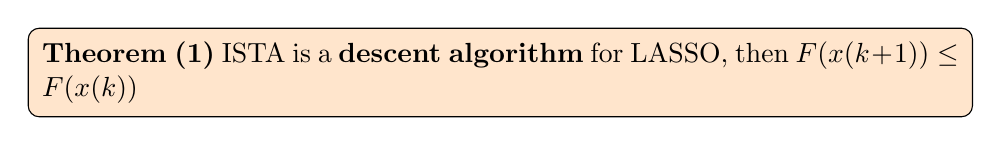
\begin{tikzpicture}
\node [mybox] (box){%
    \begin{minipage}{.96\textwidth}     %Larghezza del box
           \textbf{Theorem (1)} ISTA is a \textbf{descent algorithm} for LASSO, then $F(x(k+1))\le F(x(k))$
    \end{minipage}
};
\end{tikzpicture}

\textbf{Proof} The proof of the theorem above is very simple:
\begin{align*}
    F(x(k))=&\mathcal{R}(x(k), x(k))  \ge \quad &\text{(minimizing over x)} \\
    &\mathcal{R}(x(k+1), x(k))  \ge \quad &\text{(minimizing over b)}\\
    &\mathcal{R}(x(k+1), x(k+1)) = F(x(k+1),x(k+1))
\end{align*}

\hspace*{-5mm}
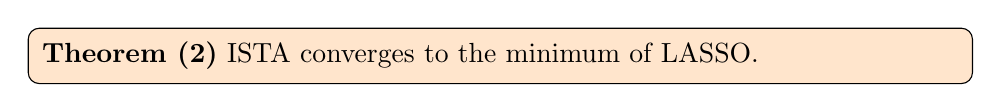
\begin{tikzpicture}
\node [mybox] (box){%
    \begin{minipage}{.96\textwidth}     %Larghezza del box
           \textbf{Theorem (2)} ISTA converges to the minimum of LASSO.
    \end{minipage}
};
\end{tikzpicture}

\subsection{Curiosity}
The equation (\ref{eq:ISTA_eq}) combines a linear part (the argument of the operator $\mathbb{S}$) and a \textbf{non linear part} that is the operator itself, being defined in a piece-wise fashion. The resulting system is a \textbf{Discrete Time Non Linear Time Invariant system} which is not trivial to treat.\\
This reminds a little the structure of a \textbf{neural network} where we have a \textbf{linear part} and a \textbf{non linear part} constituted by the \textbf{activating function}. For this reason the \textbf{evolution of ISTA} can be seen as a \textbf{Neural Network} application.

\subsection{Application of ISTA on CPS framework} 
We have seen recently that the problem of Cyber-Physical system under attacks can be formulated as follows: 
\begin{equation}
    \min_{x \in \mathbb{R}^n, a \in \mathbb{R}^q} 
    {\frac{1}{2} \bigg\lVert y-G \begin{pmatrix}
        x\\a
    \end{pmatrix} \bigg\rVert + \lambda \lVert a \rVert_1}
\end{equation}
that is a \textbf{partial LASSO} because only a part of the found solution is sparse, whose related to the (sparse) attacks. What about ISTA for Partial LASSO?
I have no limitations about the choice of the coefficient $\lambda$, in particular I can get $\lambda=0$ for the elements of the solution which are not interested by sparsity as it is the state of the system. Then, 
\begin{equation}
    \lambda\lVert a \rVert_1 = \lambda\bigg\lVert \begin{pmatrix}
        x\\a
    \end{pmatrix} \bigg\rVert_1 = 0\lvert x_1 \rvert+...+0\lvert x_n \rvert+
    \lambda \lvert a_1 \rvert + \lambda \lvert a_q \rvert
\end{equation}
This changes nothing, but it is essential that we made this variation in a way that the derivated descent algorithm could fit the "Partial LASSO" problem used for CPS purposes.


\chapter{Localization by RSS fingerprinting}
\section{Introduction}
\noindent
\textbf{Localization} is the problem related to the \textbf{estimation} of the position of a \textbf{target}. Other problems are those related to the \textbf{detection} (whether a target is present or not) and \textbf{tracking} that is we track the position of a \textbf{moving target}.\\
Nowadays the focus is in particular on \textbf{Indoor Localization} whose mathematical modeling is quite challenging due to the presence of \textit{multipath} and \textit{reflecting surfaces}. For these reasons there is not an available \textbf{unified approach}. \\
GPS is not usable for indoor localization, the so called \textbf{WSN (Wirelless Sensor Networks)} are used for this purpose. A WSN is essentially a network of devices equipped  with sensors. We can find two main approaches: 
\begin{enumerate}
    \item \textbf{Triangulation and Trilateration}: in this case we assume that the target is a \textbf{transmitting device} that broadcasts a signal. The former method deploy the \textbf{direction of arrival} of such signal, the latter use instead the \textbf{distance} from the source's signal (\textit{id est} the target). For this approach, in the case that the measurement are exact, 3 non-aligned sensors are sufficient, alternatively the higher number of sensors, the higher precision reached.
    \item \textbf{Fingerprinting methods} refers to techniques that match the \textbf{fingerprint} of some characteristics of a signal which is \textbf{location-dependent}. For our purposes we consider the \textbf{Received Signal Strength} or \textbf{RSS}.
\end{enumerate}

\section{RSS-fingerprinting: general description }
In general for all \textbf{Fingerprinting method}, we identify \textbf{two phases}:
\begin{enumerate}
    \item \textbf{Training phase} in which we collect the fingerprints of a scene; 
    \item \textbf{Runtime phase} in which we match the online measurement with the closest a-priori location fingerprints.
\end{enumerate}
As we said, we focus our attention on \textit{RSS-fingerprinting}.

\subsection{(Phase 0) Initialization }
Given the room where the localization has to be done, we deploy the WSN in some way (For example: grid deployment, or random (uniform) deployment, split the room into $p$ cells.   \textbf{Localize the target} $\longrightarrow$ detect in which cell the target is placed.

\begin{figure}[h]
    \centering
    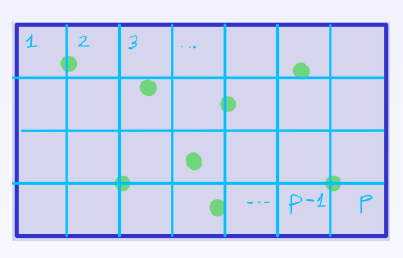
\includegraphics{images/RSS-cells.png}
    \caption{(Phase 0) - Initialization}
    \label{fig:RSS-Cells}
\end{figure}

\subsection{(Phase 1) Training phase}
We put the target in each cell. According to the fact that the target itself broadcasts a signal, \textbf{each sensor} measures and stores the RSS, and create a \textbf{signature map} or \textbf{dictionary}. More specifically, the dictionary can be represented by a matrix $D$, in which each entry $D_{i,j} $ denotes the RSS-measurement the sensor $i$ takes when the target is in the $j$-th cell. \\
\textbf{Each sensor} builds its own dictionary, and the WSN builds an \textbf{overall dictionary} $D\in \mathbb{R}^{q,p}$.\\
This phase takes some time and requires that the nodes of the network saved the information, it makes the runtime phase more accurate. 

\begin{figure}[h]
    \centering
    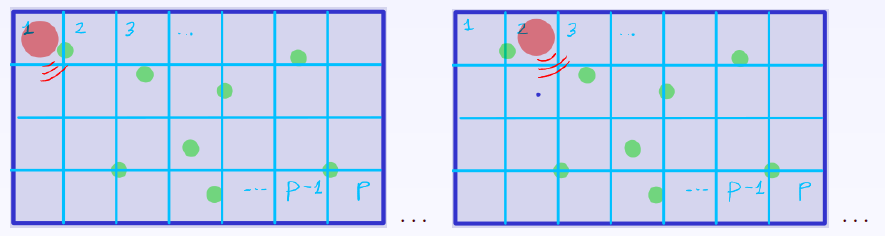
\includegraphics[scale=0.8]{images/RSS-training.png}
    \caption{(Phase 1) - Training phase}
    \label{fig:enter-label}
\end{figure}

\subsection{(Phase 2): Runtime phase}
Is the phase in which the localization is performed. Each sensor takes a measurement $y_i$, the $j$-th column of the dictionary indicates the $j$-th cell of the room in which the target is located!  

\begin{figure}[h]
    \centering
    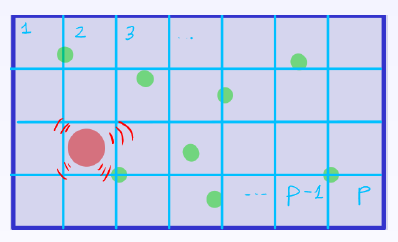
\includegraphics{images/RSS-Runtime.png}
    \caption{(Phase 2) - Runtime phase}
    \label{fig:enter-label}
\end{figure}

\noindent
If there is one target, then one of the columns of the dictionary would correspond to the measurement (in theory), then the target is located in the $j$-th cell where $j$ is such that $y=D_j$, with $D_j$ the $j-th$ column of the dictionary but usually, we can have \textit{multiple target} in the same room moreover it's very difficult that $y=D_j$ due to the presence of noise on sensors.\\

Then, in this scenario we have that the vector of measurements $y$ is a sum of a subset of the columns of the matrix $D$, to which we must add an additional term related to the noise. We have: 
\begin{equation} \label{eq: prob_loc}
	y=Dx+\text{noise}
\end{equation}
Where $x\in\{0,1\}^p$ and $x_i=1$ when in the i-th cell there is a target. \\
A further observation which can be done is that, in the real problems of \textit{indoor localization} the number of the targets one would like to localize is \textbf{much smaller} than the number of the cells, this leads to the sparsity of the solution $x\in\mathbb\{0,1\}^p$. 
Summarizing: (i) We want to find a solution to the problem (\ref{eq: prob_loc}), (ii) We know that such solution is \textbf{sparse}. Then,
\begin{equation}
	x^*=\text{arg}\min_{x\in\{0,1\}^p} \frac{1}{2} \lVert y-Dx \rVert_2^2 + \lambda \lVert x \rVert_1
 \end{equation}
This type of formulation leads to a \textbf{mixed integer} combinatorial problem, that again is NP-hard, so non-tractable. We can relax the constraint $x\in\{0,1\}^p$ into $x\in\mathbb{R}^p$, obtaining:
\begin{equation} \label{eq: loc_LASSO}
	x^*=\text{arg}\min_{x\in\mathbb{R}^p} \frac{1}{2} \lVert y-Dx \rVert_2^2 + \lambda \lVert x \rVert_1
\end{equation}
This is the problem of LASSO in the original formulation. {\color{red} It is important to remember that: } the solution of the problem (\ref{eq: loc_LASSO}) is not the original $x$ due to: (i) the presence of the noise, (ii) a bias introduced by the $\ell_1$-regularization term which in part promotes sparsity on the other hand inserts an error. One can use of course the \textbf{IST Algorithm} to find a solution.

\section{Localization under sparse sensor attacks}
\noindent
Assume that, in a realistic way, the training phase is \textit{attack-free}, therefore the matrix $D$ is attack free. Let us focus the attention again in the runtime phase.\\
What if the sensors were under adversarial attacks? One can apply the theory we developed in the former chapter! Then, we assume that the sensors under attacks are much smaller than the total number $q$ of them. In this context the equation (\ref{eq: prob_loc}) becomes: 
\begin{equation}
	y=Dx+a+noise	
\end{equation}
Then, the formulation of problem changes as follows:\\


\hspace*{-5mm}
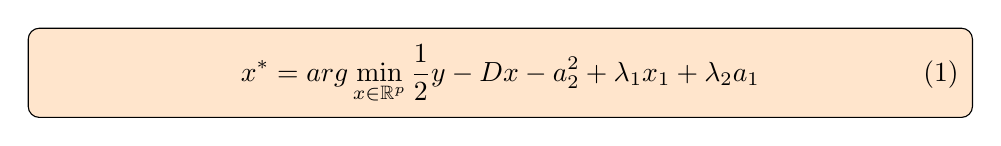
\begin{tikzpicture}
	\node [mybox] (box){%
		\begin{minipage}{.96\textwidth}     %Larghezza del box
			\begin{equation}
				x^*=\text{arg}\min_{x\in\mathbb{R}^p} \frac{1}{2} \lVert y-Dx-a \rVert_2^2 + 
				\lambda_1 \lVert x \rVert_1+
				\lambda_2\lVert a \rVert_1
			\end{equation}
		\end{minipage}
	};
\end{tikzpicture}


where we are using different weights $\lambda_1, \lambda_2$ to give more or less importance to the term related to the solution $x$ and to the attack $a$. According to this novel aspect, the risen problem is a \textbf{weighted LASSO}. \textbf{IST algorithm} continues to work, as we saw in the case of presence of \textit{non-sparse} part of the solution in the case of SSE under adversarial attacks.

\noindent
\section{Other approaches to Localization}
The approach we have just seen is not the only one. Next paragraphs are in order to give some alternatives which differ from the first we have presented in computational complexity, time of convergence and so on.

\subsection{k-Nearest Neighbour (K-NN)}
Assume to know that there is only \textbf{one target}, given the vector $y\in \mathbb{R}^q$, we could find the $j-th$ column of the dictionary $D$ that is the \textbf{nearest} with respect to $y$. The localization problem in this specific scenario becomes: 
\begin{equation} \label{eq:knn_1}
	\hat{j} = \text{arg}\min_{j=1,...,p} \lVert D_j-y \rVert_2^2
\end{equation}
where $D_j$  is the $j$-th column of $D$. Note that in the problem there is not the factor $\frac{1}{2}$ but from the moment we have a minimization problem nothing changes.\\
RSS is additive so we can localize more than one target in the \textit{runtime phase}. Suppose that the targets are $k=2$, the vector $y$ can be seen as a sum of the columns, so the problem (\ref{eq:knn_1}) gets transformed in:
\begin{equation}
	(\hat{j_1}, \hat{j_2}) = \text{arg}\min_{(j_1, j_2)=1,...,p} 
	\lVert D_{j_1}+D_{j_2}-y \rVert_2^2
\end{equation} 

In general, we have to check a number of configurations that is equal to $\binom{p}{k} \rightarrow$ \textbf{NP-Hard}. Note that: this approach can be used if we have small $p, k$ otherwise other techniques ought to be used in order to promote efficiency.

\subsection{Linear Regression (noise-free case)}
If we have multiple targets, in absence of noise the localization problem could be formulated as a \textbf{binary linear regression}. We have to solve in $x$ the equation $y=Dx$ and add the constraints about the $x$ domain and sparsity. Then, it is obtained:
\begin{equation}
	\begin{aligned}
		Dx&=y\\
		&\text{s.t.} \ x\in\{0,1\}^p, \ \sum_{j=1}^{p}x_j=k
	\end{aligned}
\end{equation}
Even in this case it has been risen a mixed-integer combinatorial problem $\rightarrow$ NP-Hard. The choice should be taken in an accurate way according to the dimension of the problem.

\section{Some comments on the setting}
These algorithms assume that there is a \textbf{Fusion Center} where data from the sensors are collected. In this way: the Fusion Center stores the whole dictionary $D$ and the runtime measurements, so that it can run the localization algorithm which is nothing but one of the exposed methods.


\chapter {Dynamic Secure State Estimation of CPSs under adversarial attacks}
It has been explained in the previous chapter that for a system 
\begin{equation} \label{eq:system}
	\begin{aligned}
		&x(k+1)=Ax(k)\\
		&y(k)=Cx(k)
	\end{aligned}
\end{equation}
if one collects $n$ measurements $y(i), i=1,..., n$, we can recover the state $x(k)$ at each $k$, if we are able to find $x(0)$ and then invert the equation
\begin{equation*}
	y = \mathcal{O}_n x(0)
\end{equation*}
the Theorem by Kalman, states that this is possible, that is the system is \textbf{observable}, if and only if $\text{rank}(\mathcal{O}_n)=n$.
This is the static-batch approach to the \textbf{state estimation problem}, on the other hand - as an alternative technique - if the system is observable we can estimate $x(k)$(then $x(0)$) dynamically by constructing a device called the \textbf{Observer}, in the deterministic case it is called \textbf{Luemberger Observer}.\\

\section{Review of Luemberger Observer}

A copy of the system (\ref{eq:system}) is made with the only difference of adding a correction term. Starting from this point we use $\hat{x}(k)$ to indicate the \textbf{estimate of the state at the time $k$} (discretized time), and $\hat{y}(k)$ is the output computed by using the estimate. The Luemberger Observer has the following equations: 
\begin{equation} \label{eq: Luemberger}
	\begin{aligned}
			&\hat{x}(k+1)=A\hat{x}(k)-L[\hat{y}(k)-y(k)]\\
		&\hat{y}(k)=C\hat{x}(k)
	\end{aligned}
\end{equation}
The quantity $e(k)=\hat{x}(k)-x(k)$ is the error of the estimate at time $k$, the aim is to design an online algorithm which could make $e(k)\rightarrow 0 $. \\
In order to understand the role of the matrix $L\in \mathbb{R}^{n,q}$,  called the \textbf{observer gain matrix}, we can write: 
\begin{align}
	e(k+1)&=\hat{x}(k)-x(k)=A\hat{x}(k)-L[\hat{y}(k)-y(k)]-Ax(k)=\\
	&=A\hat{x}(k)-LC\hat{x}(k)-LCx(k)-Ax(k)=\\
	&=A[\hat{x}(k)-x(k)]-LC[\hat{x}(k)-x(k)]=\\
	&=(A-LC) [\hat{x}(k)-x(k)]=\\
	&=(A-LC) \ e(k)	
\end{align}
The resulting equation $e(k+1)=(A-LC)\ e(k)$ describes an LTI discrete time dynamical system in which the state matrix is represented by $A-LC$. From the theory of dynamical systems, we know that the system is asymptotically (internally) stable if after a certain time $k$, it is verified that $e(k)\rightarrow 0$, the result we are seeking, it is verified when the \textit{eigenvalues} of $A-LC$ are in the unitary circle. \\

Regarding the matrix $A$ it is not very interesting to track $x(k)$ if it is asymptotically stable because in this situation $\lim_{k \to \infty} x(k)=0$. So $A$ is required to be stable but not asymptotically (some authors refers to this type of stability as \textbf{marginal stability}).\\

\hspace*{-5mm}
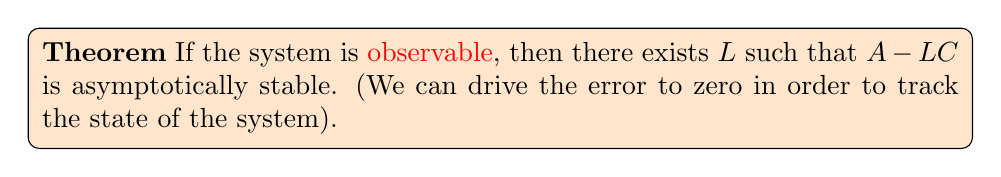
\begin{tikzpicture}
	\node [mybox] (box){%
		\begin{minipage}{.96\textwidth}     %Larghezza del box
			\textbf{Theorem} If the system is {\color{red}observable}, then there exists $L$ such that $A-LC$ is asymptotically stable. (We can drive the error to zero in order to track the state of the system).
		\end{minipage}
	};
\end{tikzpicture}

\section{State estimation by Least-squares approach}
At a certain time $k$, given the current measurement $y(k)=Cx(k)$, we might estimate $x(k)$ by solving the following problem: 
\begin{equation}
	\hat{x}(k) = \text{arg}\min_{x\in\mathbb{R}^n} \frac{1}{2} 
	\lVert y(k)-Cx \rVert_2^2 
\end{equation}
if $q>n$ and $C$ is full rank. We call $\mathcal{F}(x) =\frac{1}{2} 
\lVert y(k)-Cx \rVert_2^2$ the Least-Squares functional. 
There is a problem: the (pseudo)inversion of the matrix $C$, could be non-trivial for a medium-large dimensional problem. Even the classical Gradient Descent Algorithm would be too slow!\\
A solution is: at each $k$, we run a \textbf{single step} of gradient descent resulting in an \textbf{Online gradient descent}.\\

\hspace*{-5mm}
\begin{tikzpicture}
	\node [mybox] (box){%
		\begin{minipage}{.96\textwidth}     %Larghezza del box
				\textbf{\underline{Online Gradient Descent (OGD)}} \\
				Given the measurement $y(k)=Cx(k)$ and $\hat{x}(k)$ computed before time $k$
				\begin{align}
					\hat{x}^+(k)&=\hat{x}(k)-\tau\nabla\mathcal{F}(\hat{x}(k)) =  \hat{x}(k)-\tau C^T[C\hat{x}(k)-y(k)]\\
					&=\hat{x}(k)-\tau C^T  \ [\hat{y}(k)-y(k)] 
					\leftarrow \text{estimate of} \ x(k)\\
					\hat{x}(k+1)&=A\hat{x}^+(k) 
					\leftarrow \text{prediction of} \ x(k+1)\\
					\hat{y}(k)&=C\hat{x}(k)				
				\end{align}
		\end{minipage}
	};
\end{tikzpicture}
By merging estimate and prediction we obtain:
\begin{equation}\label{eq: OGD_obs}
	\hat{x}(k+1)=A\hat{x}(k)-\tau AC^T[\hat{y}(k)-y(k)]
\end{equation}
It can be noted that there is a certain similarity of the system (\ref{eq: OGD_obs}) and the (\ref{eq: Luemberger}), in particular the OGD is a Lumberger Observer with $L_g=\tau AC^T$.\\
Since we have fixed, in a certain way, the matrix $L_g$, one would wonder when 
\begin{equation} \label{eq:OGD_dyn}
	A-L_gC
\end{equation}
is asymptotically stable. 
We can rewrite it as $A(I-\tau C^TC)$.
If we choose $\tau<\frac{1}{\lVert C\rVert_2^2}$ then we obtain that 
$\lVert I - \tau C^TC \rVert \le 1$. Finally, two cases are to be considered: 
\begin{itemize}
	\item If $\lVert I - \tau C^TC \rVert = 1$, and A is \textit{marginally stable}, then $A-L_gC$ is marginally stable; 
	\item  If $\lVert I - \tau C^TC \rVert < 1$, and A is \textit{marginally stable}, then  $A-L_gC$ is \textbf{asymptotically stable}.
\end{itemize}

Until this moment, we have presented these results for an LTI DT dynamical system in which there are not attacks. What about \textbf{Dynamic Secure State Estimation}?

\section{Dynamic SSE with constant attack}
Recalling that a CPS under adversarial attacks on the sensors can be described by the system: 
\begin{equation}
	\begin{aligned}
		&x(k+1)=Ax(k)\\
		&y(k)=Cx(k)+a(k)
	\end{aligned}
\end{equation}
We have seen in the Second Chapter that in this case the problem of observability results in:
\begin{equation} \label{eq:CPS_attack}
	\begin{pmatrix}
		y(0)\\ \vdots \\ y(T-1)
	\end{pmatrix}=\mathcal{O}_Tx(0)+\begin{pmatrix}
	a(0) \\ \vdots \\ a(T-1)
 	\end{pmatrix}
\end{equation}
We have solved this problem for the static case in which we have seen the IST Algorithm, but in the case in which $A$ is not the identity matrix, the problem is not trivial to solve!\\
If an assumption is done on the 'shape' of the attacks the problem could be well posed, in particular we should assume that the attacks are constant and equal to a vector $a\in\mathbb{R}^q$, at this point the problem (\ref{eq:CPS_attack}) results in:
\begin{equation} 
	\begin{pmatrix}
		y(0)\\ \vdots \\ y(T-1)
	\end{pmatrix}=\mathcal{O}_nx(0)+\begin{pmatrix}
		a \\ \vdots \\ a
	\end{pmatrix} = 
	\begin{pmatrix}
		C & I\\
		CA & I \\
		\vdots & \vdots\\
		CA^{T-1} & I	
	\end{pmatrix} \begin{pmatrix}
		x(0)\\a
	\end{pmatrix}
\end{equation}
where the matrix 
\begin{equation}	\label{eq:aug_matCPS}
	\mathcal{O}_T'=\begin{pmatrix}
		C & I\\
		CA & I \\
		\vdots & \vdots\\
		CA^{T-1} & I	
	\end{pmatrix}
\end{equation}
is an \textbf{augmented observability matrix}. Is this CPS observable?\\

\noindent
In order to clarify this aspect, let us consider a couple of measurements for $k=0,1$:
\begin{align}
	&y(0)=Cx(0)+a \label{eq:first}\\ 
	&y(1)=Cx(1)+a=CAx(0)+a \label{eq:second}
\end{align}
We might manipulate algebraically these equations in order to eliminate the attack $a$ which is assumed to be constant. For example, one can subtract the (\ref{eq:second}) from the (\ref{eq:first}), and it will be obtained
\begin{align}
	&y(1)-y(0)=CAx(0) + a-Cx(0)-a=\\
	&[CA-C]x(0) =\\
	&C[A-I]x(0) \label{eq:final_equation}
\end{align} 
Moreover, let us suppose that $q=n$ so that the matrix $C[A-I]\in\mathbb{R}^{n,n}$. If such matrix would be invertible, we could recover $x(0)$ without problem by inverting the equation (\ref{eq:final_equation}). One might think that I could go further in the computation of $y(k)$ and by using such manipulations, I can eliminate the attack and recover without problems the state.\\
\underline{\textbf{BUT}} in many situations the square matrix $A-I$ is not invertible, we have seen that is reasonable that in the $\text{Spec}(A)$ (set of the eigenvalues of A) there is an eigenvalue $\lambda_i=1$ for  some $i$.
This imply that the matrix $A-I$ has a \textbf{null eigenvalue}, that is the same to confirm that the matrix is \textbf{not full rank} and for this reason \textbf{non invertible}.
One wonder if we might have a generalization of this concept. It is possible by analysing the \textbf{kernel of} $\mathcal{O}'_T$. To this aim, again, we will exploit some algebraic tricks. This time we subtract couple of rows of the matrix (\ref{eq:aug_matCPS}) from the bottom to the top, obtaining:
\begin{equation}
	\begin{pmatrix}
		C & I \\
		C(A-I) & I \\
		\vdots & \vdots \\
		CA^{T-3} (A-I) & 0\\
		CA^{T-2} (A-I) & 0
  	\end{pmatrix} \begin{pmatrix}
  		x\\a
  	\end{pmatrix}
\end{equation}
This is nothing but the system (\ref{eq:CPS_attack}) rewritten in a different form. Let us neglect at the moment the first row of the rewritten matrix. It is recognizable the matrix $\mathcal{O}_{T-1}$, however due to the fact of being multiplied by $A-I$ the linear system 
\begin{equation*}
	\mathcal{O}_{T-1}(A-I)x=0
\end{equation*}
is underdetermined and has got infinitely many solutions. Despite $\mathcal{O}_{T-1}$ is full rank (it is a minimum requirement because if the system without attack is not observable, I cannot recover the state with attacks!) we do not have a trivial kernel because of $A-I$ which is not full rank. Moreover if we add the first equation we obtain the total system
\begin{equation*}
	\begin{cases}
		(A-I)x=0\\
		Cx+a=0
	\end{cases}
\end{equation*}
We are ready to give the following proposition:\\

\hspace*{-5mm}
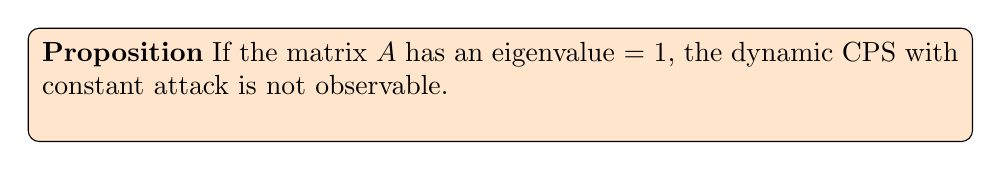
\begin{tikzpicture}
	\node [mybox] (box){%
		\begin{minipage}{.96\textwidth}     %Larghezza del box
			\textbf{Proposition} If the matrix $A$ has an eigenvalue = 1, the dynamic CPS with constant attack is not observable.\\
		\end{minipage}
	};
\end{tikzpicture}%

\noindent
The fact that an eigenvalue of A might be equal to one, is quite common from the moment we do not desire the situation in which the state tends to zero when $k\rightarrow\infty$.\\
Then, the proposition states that in general a CPS under attacks \textbf{is not observable} even if the attack is \textbf{constant}. However, we have not exploited yet the information about the \textbf{sparsity of the attacks} which allows us to develop a so-called \textbf{{\color{red} SPARSE OBSERVER}}. \\
Before giving the final result is useful to give a little of notation:
\begin{equation*}
	z(k) = \begin{pmatrix}
		x(k)\\a(k)
	\end{pmatrix}		\quad
	\hat{z}(k) = \begin{pmatrix}
		\hat{x}(k)\\\hat{a}(k)  
	\end{pmatrix}		\quad
	\hat{z}^{+}(k)=\begin{pmatrix}
		\hat{x}^+(k)\\\hat{a}^+(k)
	\end{pmatrix}		\quad
	G \ = \ (C \quad I)
\end{equation*}
We want to solve the problem of recover the state of the dynamic CPS under constant attacks that is to solve:
\begin{equation*}
	\min_{x\in\mathbb{R}^n, a \in \mathbb{R}^q}
	\frac{1}{2} \lVert y(k) - Gz(k) \rVert_2^2 + 
	\lambda \lVert a \rVert_1
\end{equation*}
It can be demonstrated that after a sufficient number $T$ of steps the solution is given by the following algorithm:\\

\hspace*{-5mm}
\begin{tikzpicture}
	\node [mybox] (box){%
		\begin{minipage}{.96\textwidth}     %Larghezza del box
			\textbf{\underline{SPARSE OBSERVER}}\\
			Given $y(k)=Gz(k)$ and $\hat{z}(k)$, 
			\begin{align*}
				\hat{z}^+(k)&=\hat{z}(k)-\tau G^T[G\hat{z}(k)-y(k)]
				& \leftarrow  \text{estimate of} \ z(k)\\
				\hat{x}(k+1) &= A\hat{x}^+(k) 
				 & \leftarrow \text{prediction of} x(k+1) \\
				 \hat{a}^(k+1) &= \mathbb{S}_{\tau\lambda}[\hat{a}^+(k)]
				 & \leftarrow \text{"sparsify" the attacks}\\
				 \hat{y}(k) &=G\hat{z}(k)
			\end{align*} 			
		\end{minipage}
	};
\end{tikzpicture}\\

\noindent
What are the differences from the previous version? The matrix $A$ is not the identity matrix, the state of the CPS \textbf{changes} $\Rightarrow$ in general $x(k) \ne x(k+1)$.


\chapter{Distributed Consensus based algorithms for CPSs}
\section{Toward the Fusion Center removal}

\section{The Consensus algorithm}

\section{Uses of the Consensus orithm}



%------------------------SECOND PART: CONTROL OF CPS---------------
\part{Control of Cyber-Physical systems}
\chapter{System identification: an introduction}
\chapter{Set-membership Identification}
\chapter{State variable feedback control (SVFB)}
\chapter{Formation contorl}
\end{document}
